\section{隆格-楞茨矢量}\label{sec:09.03}

在这一节里,我们再讨论一个守恒量,不过它不是普遍适用
的,而只适用于在引力作用下的运动。

再以太阳对行星的引力作用为例,如果取太阳的位置为坐标
原点,某行星的位置矢量为$\vec{r}$,则太阳对该行星的吸引力为
\begin{equation}\label{eqn:09.03.01}
  \vec{F} = - \frac { G M m } { r ^ { 2 } } \cdot \frac { \vec{r} } { r }
\end{equation}
其中$ M $及$ m $分别表示太阳及行星的质量$ - \frac { \vec{r} } { r }$表示力$\vec{F}$总是指向
太阳的。由牛顿第二定律,行星的运动方程应为
\begin{equation}\label{eqn:09.03.02}
  \frac { \dif ^ { 2 } r } { \dif t ^ { 2 } } = - \frac { G M } { r ^ { 2 } } \cdot \frac { \vec{r} } { r }
\end{equation}

第六章中已讨论过,行星运动中机械能是守恒的,即

% 263.jpg
\clearpage
\begin{equation}\label{eqn:09.03.03}
  T + V = E (\text{不变量})
\end{equation}
其中$ E $为行星的机械能;动能$ T $及势能$ V $分别为
\begin{align}
  T & = \frac { 1 } { 2 } m \left( \frac { \dif r } { \dif t } \right) ^ { 2 } \label{eqn:09.03.04} \\
  V & = - \frac { G M m } { r }  \label{eqn:09.03.05}
\end{align}

上节已证明,行星的角动量也是守恒的,即
\begin{equation}\label{eqn:09.03.06}
  \vec{ r } \times \vec{p} = \vec{r} \times m \frac { \dif \vec{r} } { \dif t }
  =\vec{l}\;(\text{不变量})
\end{equation}

现在,我们定义一个新的物理量$\vec{B}$,它由下式定义
\begin{equation}\label{eqn:09.03.07}
  \vec{B} = \frac { \dif \vec{r} } { \dif t } \times \vec{l} - G M m \frac { \vec{r} } { r }
\end{equation}
它称为隆格-楞茨矢量。可以证明,隆格-楞茨矢量也是一个守恒
量。证明如下:

由
\begin{equation*}
  \frac { \dif } { \dif t } \left( \frac { \dif \vec{r} } { \dif t } \times \vec{l} \right) = \frac { \dif ^ { 2 } \vec{r} } { \dif t ^ { 2 } } \times \vec{l} + \frac { \dif \vec{r} } { \dif t } \times \frac { \dif \vec{l}} { \dif t }
\end{equation*}
注意式\eqref{eqn:09.03.02}及式\eqref{eqn:09.03.06},上式成为
\begin{equation*}
  \begin{split}
    \frac { \dif } { \dif t } \left( \frac { \dif \vec{r} } { \dif t } \times \vec{l} \right) &= - \frac { G M } { r ^ { 2 } } \cdot \frac { \vec{r} } { r } \times \vec{l} \\
    &= - \frac { G M m } { r ^ { 2 } } \cdot \frac { \vec{r} } { r } \times \left( \vec{r} \times \frac { \dif \vec{r} } { \dif t } \right)
  \end{split}
\end{equation*}
利用矢量乘积公式
\begin{equation}\label{eqn:09.03.08}
  \vec{a} \times \left( \vec{b} \times \vec{c} \right) = \left( \vec{a} \cdot \vec{c} \right) \vec{b} - \left( \vec{a} \cdot \vec{b} \right) \vec{c}
\end{equation}
上式可改写成为
\begin{equation*}
  \frac { \dif } { \dif } \left( \frac { \dif \vec{r} } { \dif t } \times \vec{l} \right)
\end{equation*}
% 264.jpg
\begin{equation}\label{eqn:09.03.09}
  \begin{split}
    &= - \frac { G M m } { r ^ { 2 } } \left( \vec{r} \cdot \frac { \dif \vec{r} } { \dif t } \right) \frac { \vec{r} } { r } + \frac { G M m } { r ^ { 3 } } \left( \vec{r} \cdot \vec{r} \right) \frac { \dif \vec{r} } { \dif t } \\
    &= - \frac { G M m } { r ^ { 2 } } \left( r \frac { \dif \vec{r} } { \dif t } \right) \frac { \vec{r} } { r } + \frac { G M m } { r } \cdot \frac { \dif \vec{r} } { \dif t } \\
    &= - \frac { G M m } { r ^ { 2 } } \cdot \frac { \dif r } { \dif t } \vec{r} + \frac { G M m } { r } \cdot \frac { \dif \vec{r} } { \dif t } \\
    &= \frac { \dif } { \dif t } \left( G M m \frac { \vec{r} } { r } \right)
  \end{split}
\end{equation}
在上述推导中已经利用了下式
\begin{equation*}
  \begin{split}
    \vec{r} \cdot \frac { \dif \vec{r} } { \dif i } &= \frac { 1 } { 2 } \cdot \frac { \dif } { \dif t } \left( \vec{r} \cdot \vec{r} \right) \\
    &= \frac { 1 } { 2 } \cdot \frac { \dif } { \dif t } r ^ { 2 } \\
    &= r \frac { \dif r } { \dif t }
  \end{split}
\end{equation*}
由式\eqref{eqn:09.03.09}立即得到
\begin{equation*}
  \frac { \dif } { \dif t } \left( \frac { \dif \vec{r} } { \dif t } \times \vec{l} - G M m \frac { \vec{r} } { r } \right) = 0
\end{equation*}
即
\begin{equation}\label{eqn:09.03.10}
  \frac { \dif \vec{B} } { \dif t } = 0
\end{equation}
这就证明了$\vec{B}$的确是一个守恒量。

利用这个守恒量很容易证明开普勒第一定律,即行星的轨迹
是一椭圆形,太阳在其焦点上。

\noindent 由
\begin{equation*}
  \begin{split}
    \frac { 1 } { m } \cdot \vec{l} ^ { 2 } &= \frac { 1 } { m } \vec{l} \cdot \vec{l} \\
    &= \left( \vec{r} \times \frac { \dif \vec{r} } { \dif t } \right) \cdot \vec{l}
  \end{split}
\end{equation*}
注意矢量乘法规则

% 265.jpg
\begin{equation}\label{eqn:09.03.11}
  \begin{split}
    \vec{a} \cdot \left( \vec{b} \times \vec{c} \right) &= \vec{b} \cdot \left( \vec{c} \times \vec{a} \right) \\
    &= \vec{c} \cdot \left( \vec{a} \times \vec{b} \right)
  \end{split}
\end{equation}
上式可改写成为
\begin{equation}\label{eqn:09.03.12}
  \begin{split}
    \frac { 1 } { m } \vec{l} ^ { 2 } &= \vec{r} \cdot \left( \frac { \dif \vec{r} } { \dif t } \times \vec{l} \right) \\
    &= \vec{r} \cdot \left( \vec{B} + \frac { G M m } { r } \vec{r} \right)
  \end{split}
\end{equation}
由于$\vec{B}$是不变的矢量,故可以选为一坐标轴方向,这样就有
\begin{equation*}
  \vec{r} \cdot \vec{B} = r B \cos \varphi
\end{equation*}
其中$ \varphi $为$ \vec{r} $与$ \vec{B} $之间的夹角。用这个表达式,则式\eqref{eqn:09.03.12}可变成
\begin{equation*}
  \frac { 1 } { m } \vec{l} ^ { 2 } = r B \cos \varphi + G M m r
\end{equation*}
\begin{align}\label{eqn:09.03.13}
  \beforetext{或者} r = \frac { \vec{l} / G M m ^ 2 } { 1 + \dfrac { B } { G M m } \cos \varphi }
\end{align}
\begin{wrapfigure}[11]{r}{17em}
  \centering
  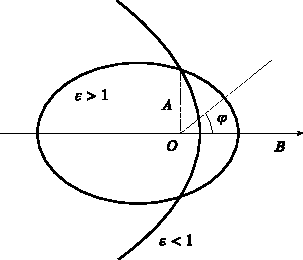
\includegraphics{figure/fig09.07}
  \caption{圆锥曲线的基本性质}
  \label{fig:09.07}
\end{wrapfigure}
这就是行星运动的轨迹。

式\eqref{eqn:09.03.13}是典型
的极坐标中的圆锥曲线
方程。根据图\ref{fig:09.07},我们
来回忆一下有关圆锥曲
线的基本性质。图中$ B $
沿极轴方向,$ \varphi $角为从
极轴计起的方位角。以
$ O $为焦点的圆锥曲线的
标准形式是
\begin{equation}\label{eqn:09.03.14}
  r = \frac { A } { 1 + \varepsilon \cos \varphi }
\end{equation}
% 266.jpg
其中$ A $为$ \varphi = \dfrac { \uppi } { 2 } $时的$ r $值,称为截距;$ \varepsilon $称为偏心率。依照偏心
率的不同,曲线\eqref{eqn:09.03.14}可分成以下几种形式:

当$ \varepsilon < 1 $时,为椭圆;

当$ \varepsilon > 1 $时,为双曲线;

当$ \varepsilon = 1 $时,为抛物线;

当$ \varepsilon = 0 $时,为圆。

这样,我们就证明了在太阳引力作用下,行星轨迹必定是圆
锥曲线,而且太阳在其焦点上。

进一步比较式\eqref{eqn:09.03.13}与式\eqref{eqn:09.03.14}还可以求得轨迹的偏心率
\begin{equation}\label{eqn:09.03.15}
  \varepsilon = \frac { B } { G M m }
\end{equation}
根据$ \vec{B} $的定义式\eqref{eqn:09.03.07},$\vec{B}$的大小可以按下面的方法求出:
\begin{equation*}
  \begin{split}
    B ^ { 2 } =& \vec{B} \cdot \vec{B} \\
    =& \left( \frac { \dif \vec{r} } { \dif t } \times \vec{l} - G M m \frac { \vec{r} } { r } \right) \cdot \left( \frac { \dif \vec{r} } { \dif t } \times \vec{l} - G M m \frac { \vec{r} } { r } \right) \\
    =& \left( \frac { \dif \vec{r} } { \dif t } \times \vec{l} \right) \cdot \left( \frac { \dif \vec{r} } { \dif t } \times \vec{l} \right) \\
    & - 2 G M m \frac { \vec{r} } { r }  \cdot \left( \frac { \dif \vec{r} } { \dif t } \times \vec{l} \right) + \left( G M m \right) ^ { 2 }
  \end{split}
\end{equation*}
利用公式\eqref{eqn:09.03.08}及式\eqref{eqn:09.03.11},上式能化简成为
\begin{equation*}
  \begin{split}
    B ^ { 2 } =& \left[ \left( \frac { \dif \vec{r} } { \dif t } \times \vec{l} \right) \times \frac { \dif \vec{r} } { \dif t } \right] \cdot \vec{ l } \\
    &- 2 G M m \frac { \vec{r} } { r }  \cdot \left( \frac { \dif \vec{r} } { \dif t } \times \vec{l} \right) + \left( G M m \right) ^ { 2 } \\
    =& \frac { 2 } { m } \left[ \frac { 1 } { 2 } m \left( \frac { \dif \vec{r} } { \dif t } \right) ^ { 2 } - \frac { G M m } { r } \right] l ^ { 2 } + \left( G M m \right) ^ { 2 }
  \end{split}
\end{equation*}

% 267.jpg
\clearpage\noindent 再由能量守恒公式\eqref{eqn:09.03.03}、\eqref{eqn:09.03.04}、\eqref{eqn:09.03.05},上式可表示为
\begin{equation}\label{eqn:09.03.16}
  B ^ { 2 } = \frac { 2 } { m } E l ^ { 2 } + G ^ { 2 } M ^ { 2 } m ^ { 2 }
\end{equation}
代入式\eqref{eqn:09.03.15}即得
\begin{equation}\label{eqn:09.03.17}
  \begin{split}
    \varepsilon &= \frac { B } { G M m } \\
    &= \left( 1 + \frac { 2 E l ^ { 2 } } { G ^ { 2 } M ^ { 2 } m ^ { 3 } } \right) ^ { \frac { 1 } { 2 } }
  \end{split}
\end{equation}

总之,隆格-楞茨矢量$ \vec{B} $的物理意义是:

(1)其方向指向行星轨道最靠近太阳的点,常简称指向近日
点

(2)它的大小决定轨道的偏心率。

由式\eqref{eqn:09.03.17}可以看到,只有当$ E<0 $时,轨迹才可能是椭
圆(即$ \varepsilon < 1 $),因此,行星的机械能\lhbrak 按式\eqref{eqn:09.03.03}所给定的数\rhbrak 必
定小于零;当$ E > 0 $时,$ \varepsilon > 1 $,运动轨迹是双曲线,它不是周期
性的运动,而是从无限远来再到无限远去的运动。

圆轨道的条件是$ \varepsilon = 0 $,即应有
\begin{equation}\label{eqn:09.03.18}
  1 + \frac { 2 E l ^ { 2 } } { G ^ { 2 } M ^ { 2 } m ^ { 3 } } = 0
\end{equation}
这个结果说明,对于圆运动,行星的机械能与其角动量$ l $之间具
有确定的关系,相互不是独立的。实际上式\eqref{eqn:09.03.18}可由能量守
恒式\eqref{eqn:09.03.03}和角动量守恒式\eqref{eqn:09.03.06}直接得到。因为在圆运动情况
\begin{equation*}
  l = m r v
\end{equation*}
以及
\begin{equation*}
  v ^ { 2 } = \frac { G M } { r }
\end{equation*}
将上两式代入能量守恒公式
\begin{equation*}
  \frac { 1 } { 2 } m v ^ { 2 } - \frac { G M m } { r } = E
\end{equation*}
% 268.jpg
即可得到式\eqref{eqn:09.03.18}。

\example 一个质量为$ m $的宇宙飞船,环绕一个行星作圆轨道
运动,轨道半径为$ R _ 0 $,飞船速率为$ v _ 0 $。突然点燃一个火箭,使飞
船增加了向外的径向速度分量$ v _ r $(设$ v _ r < v _ 0$),因此飞船的轨道变
成椭圆形。

(1)用$ R _ { 0 }  , v _ { 0 }  $表示出引力$ F $的表达式;

(2)用$ R _ { 0 } , v _ { 0 }  , v _ { r }  $表示出新轨道方程,并画出$ v _ { r } = \dfrac { 1 } { 2 } v _ { 0 } $时的
轨道草图;

(3)求新轨道的半长轴$ a $,并证明,对于原来的圆轨道和新
的椭圆轨道,$ Ea $是相同的($ E $为总能量)。

\solution (1)对于圆轨道,有
\begin{equation*}
  \frac { G M m } { R _ 0 ^ { 2 } } = m \frac { v _ 0 ^ { 2 } } { R _ { 0 } }
\end{equation*}
\begin{align*}
  \beforetext{即} &G M m = m v _ 0 ^ { 2 } R _ { 0 } = C \\
  \beforetext{故} &| F | = \frac { m v _ 0 ^ { 2 } R _ { 0 } } { r ^ { 2 } }
\end{align*}
式中$ r $是在此引力场内某点与力心的距离。

(2)火箭点燃,角动量不变
\begin{equation*}
  l = m v _ { 0 } R _ { 0 }
\end{equation*}
是守恒量。而新能量值为
\begin{equation*}
  \begin{split}
    E ^ { \prime } &= E _ { K } + E _ { P } \\
    &= \left( \frac { 1 } { 2 } m v _ 0 ^ { 2 } + \frac { 1 } { 2 } m v _ r ^ { 2 } \right) - \frac { G M m } { R _ { 0 } } \\
    &= \frac { 1 } { 2 } m v _ 0 ^ { 2 } + \frac { 1 } { 2 } m v _ r ^ { 2 } - m v _ 0 ^ { 2 } \\
    &= - \frac { 1 } { 2 } m v _ 0 ^ { 2 } + \frac { 1 } { 2 } m v _ r ^ { 2 }
  \end{split}
\end{equation*}
% 269.jpg
根据式\eqref{eqn:09.03.17}新的偏心率为
\begin{equation*}
  \begin{split}
    \varepsilon ^ { \prime } &= \left( 1 + \frac { 2 E ^ { \prime } l ^ { 2 } } { m C ^ { 2 } } \right) ^ { \frac { 1 } { 2 } } \\
    &= \left( 1 - 1 + \frac { v _ { r } ^ { 2 } } { v _ 0 ^ { 2 } } \right) ^ { \frac { 1 } { 2 } } \\
    &= \frac { v _ { r } } { v _ { 0 } }
  \end{split}
\end{equation*}
新的参量$ A ' $为
\begin{equation*}
  \begin{split}
    A ^ { \prime } &= \frac { l ^ { 2 } } { m C } \\
    &= \frac { m ^ { 2 } v _ 0 ^ { 2 } R _ 0 ^ { 2 } } { m m v _ 0 ^ { 2 } R _ { 0 } } \\
    &= R _ { 0 }
  \end{split}
\end{equation*}
故得新的轨道方程
\begin{equation*}
  \begin{split}
    r &= \frac { R _ { 0 } } { 1 + \varepsilon ^ { \prime } \cos \varphi } \\
    &= \frac { R _ { 0 } } { 1 + \dfrac {  v _ { r } } { v _ { 0 } } \cos \varphi }
  \end{split}
\end{equation*}
当$ v _ { r } = \dfrac { 1 } { 2 } v _ { 0 } $时,轨道方程为
\vspace{-0.5em}
\begin{figure}[h]
  \centering
  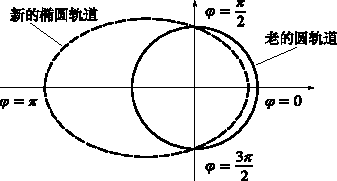
\includegraphics{figure/fig09.08}
  \caption{}
  \label{fig:09.08}
\end{figure}
% 270.jpg
\begin{equation*}
  r = \frac { R _ { 0 } } { 1 + \dfrac { 1 } { 2 } \cos \varphi }
\end{equation*}
此时轨道的草图如图\ref{fig:09.08}所示。

(3)长轴$ 2 a = r \left( \varphi = 0 \right) + r \left( \varphi = \uppi \right) $
\begin{equation*}
  \begin{split}
    2 a &= \frac { R _ { 0 } } { 1 + \varepsilon ^ { \prime } } + \frac { R _ { 0 } } { 1 - \varepsilon ^ { \prime } }  \\
    &= \frac { 2 R _ { 0 } } { 1 - \varepsilon ^ { \prime 2 } } \\
    &= \frac { 2 R _ { 0 } } { 1 - \left( \dfrac { v _ { r } } { v _ { 0 } } \right) ^ { 2 }}
  \end{split}
\end{equation*}
对于
\begin{align*}
  v _ { r } & = \frac { 1 } { 2 } v _ { 0 } \\
  a         & = \frac { 4 } { 3 } R _ { 0 }
\end{align*}
对于新轨道,
\begin{equation*}
  \begin{split}
    E^{\prime} a &=\left(-\frac{1}{2} m v_{0}^{2}+\frac{1}{2} m v_{r}^{2}\right) \frac{R_{0}}{1-\left(\dfrac{v_{r}}{v_{0}}\right)^{2}} \\
    &=-\frac{1}{2} m v_{0}^{2} R_{0}
  \end{split}
\end{equation*}
对于老轨道,
\begin{equation*}
  \begin{split}
    E a &= E R _ { 0 } \\
    &= - \frac { 1 } { 2 } m v _ 0 ^ { 2 } R _ { 0 }
  \end{split}
\end{equation*}
两者相同,因此得证。


\example 宇宙飞船绕一行星作圆轨道飞行,轨道半径为$ R _ 0 $,

% 271.jpg
\clearpage\noindent 飞行速率为$ v _ { 0 } $。船长想把轨道改变为经过$ B $点的椭圆形,$ B $点距
\begin{wrapfigure}[9]{r}{17em}
  \centering
  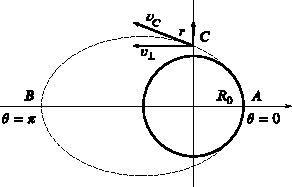
\includegraphics{figure/fig09.09}
  \caption{}
  \label{fig:09.09}
\end{wrapfigure}
行星中心为$ 3 R _ { 0 } $,如图\ref{fig:09.09}所示。

(1)写出椭圆的轨道方程。为了使飞船进入这个轨道,飞船在$ A $
点的速率必须增为多少?

(2)从$ A $到$ B $的航行,要多少时间?


(3)求飞船在$ C $点的速度沿椭圆长轴的速度分量$ v _ \bot $和$ \dot{ r } $。

\solution (1)由圆轨道,有
\begin{equation*}
  \begin{split}
    G M m &= m v _ 0 ^ { 2 } R _ { 0 } \\
    &= C
  \end{split}
\end{equation*}
所期望的轨道是
\begin{align*}
  r _ { \symrm{ min } } & = \frac { A } { 1 + \varepsilon } = R _ { 0 }   \\
  r _ { \symrm{ max } } & = \frac { A } { 1 - \varepsilon } = 3 R _ { 0 }
\end{align*}
求解得到
\begin{align*}
  \varepsilon & = \frac { 1 } { 2 }           \\
  A           & = \frac { 3 } { 2 } R _ { 0 }
\end{align*}
故轨道方程为
\begin{equation*}
  r = \frac { \dfrac { 3 } { 2 } R _ { 0 } } { 1 + \dfrac { 1 } { 2 } \cos \varphi }
\end{equation*}
% 272.jpg
根据$ A , \varepsilon $的定义\lhbrak 式\eqref{eqn:09.03.13}及式\eqref{eqn:09.03.17}\rhbrak ,再由长轴的定义,
有
\begin{equation*}
  \begin{split}
    2 a &= 4 R _ { 0 } \\
    &= \frac { 2 A } { 1 - \varepsilon ^ { 2 } } \\
    &= \frac { \dfrac { 2 l ^ { 2 } } { m G } } { 1 - \left( 1 + \dfrac { 2  E ^ { \prime } l ^ { 2 } } { m C ^ { 2 } } \right) }\\
    &= - \frac { C ^ { 2 } } { E ^ { \prime } }
  \end{split}
\end{equation*}
即
\begin{equation*}
  \begin{split}
    E ^ { \prime } &= - \frac { C ^ { 2 } } { 4 R _ { 0 } } \\
    &= - \frac { m v _ 0 ^ { 2 } R _ { 0 } } { 4 R _ { 0 } } \\
    &= - \frac { 1 } { 4 } m v _ { 0 } ^ 2
  \end{split}
\end{equation*}
由$ E ^ { \prime } $的定义,在$ A $点有
\begin{equation*}
  \begin{split}
    E ^ { \prime } &= \frac { 1 } { 2 } m v _ A ^ { 2 } - \frac { C } { R _ { 0 } } \\
    &=  \frac { 1 } { 2 } m v _ A ^ { 2 } - m v _ 0 ^ { 2 }
  \end{split}
\end{equation*}
由此得飞船在$ A $点的速率增加为
\begin{equation*}
  v _ { A } = \sqrt { \frac { 3 } { 2 } } v _ { 0 }
\end{equation*}

(2)利用开普勒定律\lhbrak 式\eqref{eqn:09.02.05}\rhbrak 有
\begin{equation*}
  \frac { \dif A ^ { \prime } } { \dif t } = \frac { l } { 2 m }
\end{equation*}
% 273.jpg
周期之比为

~\vspace{-1.56em}
\begin{equation*}
  \frac { T _ { 2 } } { T _ { 1 } } = \Bigg( \frac { A _ 2 ^ { \prime } } { A _ { 1 } } \Bigg) \Bigg( \frac { l _ { 1 } } { l _ { 2 } } \Bigg) \Bigg( \frac { m } { m } \Bigg)
\end{equation*}
已知%\vspace{-1.56em}
\begin{equation*}
  \begin{split}
    T _ { 1 } &= \frac { 2 \uppi R _ { 0 } } { v _ { 0 } }  \\
    A _ 1 ^ { \prime } &= \uppi R _ 0 ^ { 2 } \\
    A _ 2 ^ { \prime } &= \uppi a b \\[-0.5em]
    &= \uppi \left( 2 R _ 0 \right) \frac { \dfrac { 3 } { 2 } R _ { 0 } } { \sqrt { 1 - \left( \dfrac { 1 } { 2 } \right) ^ { 2 } } } \\
    &= 2 \uppi \sqrt { 3 } R _ 0 ^ { 2 } \\
    T _ { 2 } &= \frac { 2 \uppi R _ { 0 } } { v _ { 0 } } \Biggl( \frac { 2 \uppi \sqrt { 3 } R _ { 0 } ^ { 2 } }  { \uppi R _ { 0 } ^ { 2 } } \Biggr) \Biggl( \frac { v _ 0  } { \sqrt { \dfrac { 3 } { 2 } } v _ { 0 } } \Biggr) \\[-0.5em]
    &= \frac { 4 \sqrt { 2 } \uppi R _ { 0 } } { v _ { 0 } }
  \end{split}
\end{equation*}
故从$ A $到$ B $的时间为
\begin{equation*}
  \begin{split}
    T &= \frac { 1 } { 2 } T _ { 2 } \\
    &= \frac { 2 \sqrt { 2 } \uppi R _ { 0 } } { v _ { 0 } }
  \end{split}
\end{equation*}

(3)爆发之后,在$ A $点有
\begin{equation*}
  \begin{split}
    E ^ { \prime } &= - \frac { 1 } { 4 } m v _ 0 ^ { 2 } \\
    l ^ { \prime } &= l _ { 2 } \\
    &= m v _ { A } R _ { 0 } \\
    &= m \sqrt { - \frac { 3 } { 2 } } v _ { 0 } R _ { 0 }
  \end{split}
\end{equation*}

% 274.jpg
\clearpage\noindent $ E ^ { \prime } $和$ l ^ { \prime } $是不变的,在$ C $点, $ \theta = \dfrac { \uppi } { 2 } $ , $ r = \dfrac { 3 } { 2 } R _ { 0 } $ ,故
\begin{equation*}
  \begin{split}
    l ^ { \prime } &= m \sqrt { \frac { 3 } { 2 } } v _ { 0 } R _ { 0 } \\
    &= m v _ { \bot } \left( \frac { 3 } { 2 } R _ { 0 } \right) \\
    E ^ { \prime } &= - \frac { 1 } { 4 } m v _ 0 ^ { 2 } \\
    &= \frac { 1 } { 2 } m \dot { r } ^ { 2 } + \frac { 1 } { 2 } m v _ { \bot } ^ { 2 } - \frac { C } { \dfrac { 3 } { 2 } R _ { 0 } } \\
    &= \frac { 1 } { 2 } m \dot { r } ^ { 2 } + \frac { 1 } { 2 } m v _ { \bot } ^ { 2 } - \frac { m v _ 0 ^ 2 R _ 0 } { \dfrac { 3 } { 2 } R _ { 0 } }
  \end{split}
\end{equation*}
解上两式得
\begin{equation*}
  \begin{split}
    v _ { \bot } &= \sqrt { \frac { 2 } { 3 } } v _ { 0 } \\
    \dot { r } &= \sqrt { \frac { 1 } { 6 } } v _ { 0 }
  \end{split}
\end{equation*}
